\chapter{Arhitektura i dizajn sustava}
		
		\textbf{\textit{dio 1. revizije}}\\

		\textit{ Potrebno je opisati stil arhitekture te identificirati: podsustave, preslikavanje na radnu platformu, spremišta podataka, mrežne protokole, globalni upravljački tok i sklopovsko-programske zahtjeve. Po točkama razraditi i popratiti odgovarajućim skicama:}
	\begin{itemize}
		\item 	\textit{izbor arhitekture temeljem principa oblikovanja pokazanih na predavanjima (objasniti zašto ste baš odabrali takvu arhitekturu)}
		\item 	\textit{organizaciju sustava s najviše razine apstrakcije (npr. klijent-poslužitelj, baza podataka, datotečni sustav, grafičko sučelje)}
		\item 	\textit{organizaciju aplikacije (npr. slojevi frontend i backend, MVC arhitektura) }		
	\end{itemize}

	
		

		

				
		\section{Baza podataka}
			
			\textbf{\textit{dio 1. revizije}}\\
			
		\textit{Podaci u našoj aplikaciji će se spremati u relacijsku bazu podataka koristeći Postgres kao DBMS. Baza će se sastojati od sljedećih entiteta:}
		\begin{itemize}
			\item Korisnik
			\item Tvrtka
			\item Projekt
			\item KategorijaProjekta
			\item ProjectFrTeamMembers
			\item Grad
			\item Zaposlenik
			\item Suradnja
		\end{itemize}
			\subsection{Opis tablica}

				\begin{longtblr}[
					label=none,
					entry=none
					]{
						width = \textwidth,
						colspec={|X[14,l]|X[8, l]|X[20, l]|}, 
						rowhead = 1,
					} %definicija širine tablice, širine stupaca, poravnanje i broja redaka naslova tablice
						\hline \multicolumn{3}{|c|}{\textbf{Korisnik}}	 \\ \hline[3pt]
						\SetCell{LightGreen}IDKorisnik & INT & ID kosisnika  	\\ \hline
						Ime	& VARCHAR & Ime korisnika \\ \hline 
						Prezime & VARCHAR & Prezime korisnika \\ \hline 
						NickName & VARCHAR	& Nadimak korisnika \\ \hline 
                    				LoginEmail & VARCHAR	& Email adresa pomoću kojeg se user logira \\ \hline 
                    				NotificationEmail & VARCHAR	& Email adresa na koju korisnik prima obavijesti \\ \hline 
						MaxRazinaOvlasti & INT & Maksimalna razina ovlasti na projektima \\ \hline
				\end{longtblr}

				\begin{longtblr}[
					label=none,
					entry=none
					]{
						width = \textwidth,
						colspec={|X[14,l]|X[8, l]|X[20, l]|}, 
						rowhead = 1,
					} %definicija širine tablice, širine stupaca, poravnanje i broja redaka naslova tablice
						\hline \multicolumn{3}{|c|}{\textbf{Tvrtka}}	 \\ \hline[3pt]
						\SetCell{LightGreen} IdTvrtka & INT	&  Id tvrtke	\\ \hline
						Naziv & VARCHAR & Naziv tvrtke \\ \hline 
						Podrucje & VARCHAR &  Područje kojim se tvrtka bavi \\ \hline 
						ABCKategorija & CHAR & Kategorija tvrtke (A B ili C) \\ \hline 
				                MjesecPlaniranjaBudzeta & INT & Mjesec u kojem tvrtka planira budžet \\ \hline
				                Drzava & VARCHAR & Država u kojoj tvrtka posluje \\ \hline
				                \SetCell{LightBlue} PostanskiBr & VARCHAR & Poštanski broj grada tvrtke \\ \hline
						Adresa & VARCHAR & Adresa sjedišta tvrtke \\ \hline
	    		                 	WebStranica & VARCHAR & Adresa web stranice tvrtke \\ \hline
				                Kontaktirati & BOOLEAN & Da li ubuduće tu tvrtku treba kontaktirati \\ \hline
				\end{longtblr}

				\begin{longtblr}[
					label=none,
					entry=none
					]{
						width = \textwidth,
						colspec={|X[14,l]|X[8, l]|X[20, l]|}, 
						rowhead = 1,
					} %definicija širine tablice, širine stupaca, poravnanje i broja redaka naslova tablice
					\hline \multicolumn{3}{|c|}{\textbf{Projekt}}	 \\ \hline[3pt]
					\SetCell{LightGreen}IDProjekt & INT	& Id projekta \\ \hline
					Naziv & VARCHAR & Naziv projekta \\ \hline 
					\SetCell{LightBlue} KategorijaProjekta & INT & Kategorija projekta \\ \hline 
					TipProjekta & VARCHAR & Eksterni ili interni projekt \\ \hline 
					Pocetak & TIMESTAMP & Datum početka projekta \\ \hline 
			                Završetak & TIMESTAMP & Datum završetka projekta \\ \hline 
			                \SetCell{LightBlue} FrResponsibleUserId & INT & Id FR responsible usera \\ \hline
			                FRCilj & FLOAT & Količina novca koja se želi prikupiti za projekt \\ \hline
			                FirstPing & TIMESTAMP & Trenutak prvog "ping"-a \\ \hline
			                SecondPing & TIMESTAMP & Trenutak drugog "ping"-a \\ \hline
				\end{longtblr}

				\begin{longtblr}[
					label=none,
					entry=none
					]{
						width = \textwidth,
						colspec={|X[14,l]|X[8, l]|X[20, l]|}, 
						rowhead = 1,
					} %definicija širine tablice, širine stupaca, poravnanje i broja redaka naslova tablice
					\hline \multicolumn{3}{|c|}{\textbf{TipProjekta}}	 \\ \hline[3pt]
					\SetCell{LightGreen}IDTipProjekt & INT	& Id tipa projekta \\ \hline
					TipProjekta	& VARCHAR & Tip projekta \\ \hline 
				\end{longtblr}

				\begin{longtblr}[
					label=none,
					entry=none
					]{
						width = \textwidth,
						colspec={|X[14,l]|X[8, l]|X[20, l]|}, 
						rowhead = 1,
					} %definicija širine tablice, širine stupaca, poravnanje i broja redaka naslova tablice
					\hline \multicolumn{3}{|c|}{\textbf{ProjectFrTeamMembers}}	 \\ \hline[3pt]
					\SetCell{LightGreen}IDKorisnik & INT & Id korisnika koji je FR team member projekta \\ \hline
					\SetCell{LightGreen}IDProjekt & INT & Id projekta \\ \hline
				\end{longtblr}

				\begin{longtblr}[
					label=none,
					entry=none
					]{
						width = \textwidth,
						colspec={|X[14,l]|X[8, l]|X[20, l]|}, 
						rowhead = 1,
					} %definicija širine tablice, širine stupaca, poravnanje i broja redaka naslova tablice
					\hline \multicolumn{3}{|c|}{\textbf{Grad}}	 \\ \hline[3pt]
					\SetCell{LightGreen} PostanskiBrojGrad & VARCHAR & Poštanski broj grada \\ \hline
					NazivGrad & VARCHAR & Naziv grada \\ \hline
				\end{longtblr}

				\begin{longtblr}[
					label=none,
					entry=none
					]{
						width = \textwidth,
						colspec={|X[14,l]|X[8, l]|X[20, l]|}, 
						rowhead = 1,
					} %definicija širine tablice, širine stupaca, poravnanje i broja redaka naslova tablice
					\hline \multicolumn{3}{|c|}{\textbf{Zaposlenik}}	 \\ \hline[3pt]
						\SetCell{LightGreen} IDZaposlenik & INT	& Id zaposlenika \\ \hline
						\SetCell{LightBlue} IDTvrtke & INT & Id tvrtke za koju zaposlenik radi\\ \hline 
						Ime & VARCHAR & Ime zaposlenika \\ \hline 
						Prezime & VARCHAR	& Prezime zaposlenika \\ \hline 
			                    Email & VARCHAR	& Email adresa zaposlenika \\ \hline 
			                    BrojTelefona & VARCHAR	& Broj telefona zaposlenika \\ \hline 
			                    Uloga & VARCHAR	& Uloga zaposlenika u tvrtci (npr. CEO) \\ \hline 
			                    Opis & VARCHAR	& Opis zaposlenika (npr. glavni kontakt) \\ \hline 
				\end{longtblr}

				\begin{longtblr}[
					label=none,
					entry=none
					]{
						width = \textwidth,
						colspec={|X[14,l]|X[8, l]|X[20, l]|}, 
						rowhead = 1,
					} %definicija širine tablice, širine stupaca, poravnanje i broja redaka naslova tablice
					\hline \multicolumn{3}{|c|}{\textbf{Suradnja}}	 \\ \hline[3pt]
					\SetCell{LightGreen}IDProjekt & INT	& Id projekta \\ \hline
			                \SetCell{LightGreen}IdTvrtke & INT	& Id tvrtke \\ \hline
					\SetCell{LightBlue}IdKontakt & INT & Id kontakt osobe u tvrtci \\ \hline 
					KategorijaSuradnje & VARCHAR & Kategorija suradnje (Financijska, materijalna ili akademska) \\ \hline
		                    Status & VARCHAR & Kontaktirano, ping, dopis, sastanak, uspješno ili neuspješno \\ \hline
		                    VrijednostSuradnje & FLOAT & Novčana vrijednost suradnje \\ \hline
				\end{longtblr}
				
			
			\subsection{Dijagram baze podataka}
				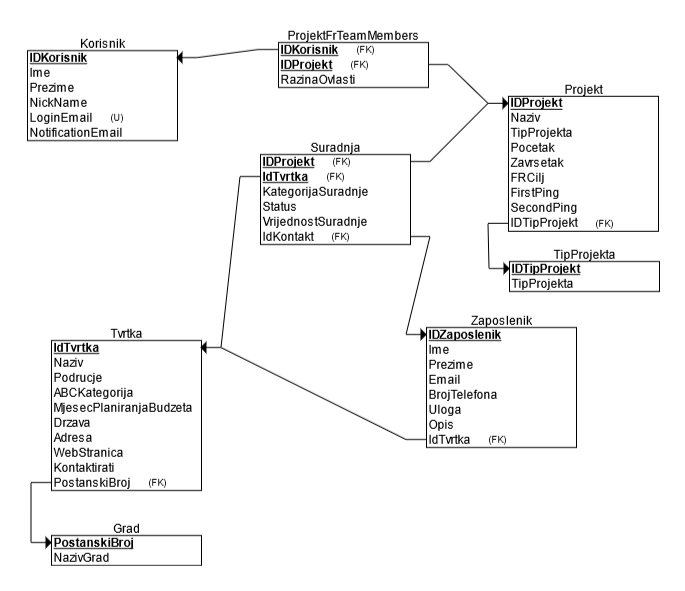
\includegraphics[scale=0.5]{DBDiagram}
			
			\eject
			
			
		\section{Dijagram razreda}
		
			\textit{Potrebno je priložiti dijagram razreda s pripadajućim opisom. Zbog preglednosti je moguće dijagram razlomiti na više njih, ali moraju biti grupirani prema sličnim razinama apstrakcije i srodnim funkcionalnostima.}\\
			
			\textbf{\textit{dio 1. revizije}}\\
			
			\textit{Prilikom prve predaje projekta, potrebno je priložiti potpuno razrađen dijagram razreda vezan uz \textbf{generičku funkcionalnost} sustava. Ostale funkcionalnosti trebaju biti idejno razrađene u dijagramu sa sljedećim komponentama: nazivi razreda, nazivi metoda i vrste pristupa metodama (npr. javni, zaštićeni), nazivi atributa razreda, veze i odnosi između razreda.}\\
			
			\textbf{\textit{dio 2. revizije}}\\			
			
			\textit{Prilikom druge predaje projekta dijagram razreda i opisi moraju odgovarati stvarnom stanju implementacije}
			
			
			
			\eject
		
		\section{Dijagram stanja}
			
			
			\textbf{\textit{dio 2. revizije}}\\
			
			\textit{Potrebno je priložiti dijagram stanja i opisati ga. Dovoljan je jedan dijagram stanja koji prikazuje \textbf{značajan dio funkcionalnosti} sustava. Na primjer, stanja korisničkog sučelja i tijek korištenja neke ključne funkcionalnosti jesu značajan dio sustava, a registracija i prijava nisu. }
			
			
			\eject 
		
		\section{Dijagram aktivnosti}
			
			\textbf{\textit{dio 2. revizije}}\\
			
			 \textit{Potrebno je priložiti dijagram aktivnosti s pripadajućim opisom. Dijagram aktivnosti treba prikazivati značajan dio sustava.}
			
			\eject
		\section{Dijagram komponenti}
		
			\textbf{\textit{dio 2. revizije}}\\
		
			 \textit{Potrebno je priložiti dijagram komponenti s pripadajućim opisom. Dijagram komponenti treba prikazivati strukturu cijele aplikacije.}